% --- Chapter appendices ---------------------------------
\renewcommand{\thesection}{\thechapter.\Alph{section}}
\setcounter{section}{0}

\section{Extended absorption models}
\label{m:app:moc-extended}

This appendix records the absorption-only and absorption--birth--death
developments that support \cref{m:sec:moc} but are not required for the single worked
example in the main text.

\subsection{Absorption only}
\label{m:sec:absonly}

The simplest absorption process has a single compartment that takes in particles,
with no subsequent dynamics: no birth and no death within the compartment.

Let $X_t$ and $Y_t$ count the particles inside and outside the compartment
respectively; the same labelling is used for every version of the
single-compartment model below. Events are stochastic with exponentially
distributed inter-event times, which by \cref{m:sec:exp} follows from the assumption
that event rates do not depend on time, so that $\{(X_t,Y_t):t\ge0\}$ is a
continuous-time Markov chain in the sense of \cref{m:sec:ctmc}.

With only absorption to consider, the model is specified by the transition
probabilities over an infinitesimal interval $\Delta t$,
\begin{align*}
\pr{\Delta X = 1,\ \Delta Y = -1 \mid Y_t = j} &= j\alpha\,\Delta t, &&\text{(absorption)}\\
\pr{\Delta X = 0,\ \Delta Y = 0 \mid Y_t = j} &= 1-j\alpha\,\Delta t, &&\text{(no event)}
\end{align*}
where $\Delta X = X_{t+\Delta t}-X_t$ and similarly for $Y$, and terms of
$o(\Delta t)$ are suppressed throughout. The factor $j$ records that each exterior
particle is independently subject to the same probability $\alpha\Delta t$ of being
taken up. The initial condition is $X_0=0$, $Y_0=N$: a starter population of $N$
particles occupying the exterior medium.

Writing $p_{i,j}(t) = \pr{X_t=i,\ Y_t=j}$, the forward Kolmogorov equations are
\begin{equation}
\label{m:eq:FK1}
\ddt{p_{i,j}} = \alpha(j+1)p_{i-1,j+1} - \alpha j\,p_{i,j} .
\end{equation}
With the bivariate generating function
\begin{equation}
\label{m:eq:pgfDef}
G(x,y,t) = \sum_i\sum_j p_{i,j}(t)\,x^iy^j = \ex{x^{X_t}y^{Y_t}},
\end{equation}
\cref{m:eq:FK1} converts into a partial differential equation by the procedure of
\cref{m:sec:pgf}. Multiply each equation by $x^iy^j$ and sum over $i$ and $j$; the
sums are finite, because $p_{i,j}(t)=0$ whenever $i+j\neq N$, particles in this
model being neither created nor destroyed. Shifting indices in the first term
sends $\alpha(j+1)p_{i-1,j+1}x^iy^j$ to $\alpha x\,\partial_yG$, and the second
term is $-\alpha y\,\partial_yG$, so that
\begin{equation}
\label{m:eq:PDE1}
\pddt{G} = \alpha(x-y)\pdd{G}{y},
\qquad G(x,y,0) = y^N .
\end{equation}

This first-order linear initial value problem is more awkward than it looks. The
method of characteristics applies in principle to equations in three variables, but
applying it here is not straightforward, and it is postponed to
\cref{m:sec:mocabsdeath}. The solution can be obtained by other means, and it is
worth doing so both because the answer is needed and because it provides a check on
the machinery developed there.

\subsubsection*{Exploiting independence}

The function $G$ above was specific to $X_0=0$, $Y_0=N$. Define more generally
\begin{equation*}
G_n(x,y,t) = \sum_i\sum_j\pr{X_t=i,\ Y_t=j \mid X_0=0,\ Y_0=n}\,x^iy^j .
\end{equation*}
In a process of pure absorption the $n$ particles are taken up one by one, and the
behaviour of any one of them does not depend on the movements of its neighbours.
That independence lets $X_t$ and $Y_t$ decompose into sums of $n$ single-particle
variables,
\begin{equation*}
X_t = \sum_{k=1}^{n}X_t^{(k)},
\qquad
Y_t = \sum_{k=1}^{n}Y_t^{(k)},
\end{equation*}
from which
\begin{equation}
\label{m:eq:indRelPGF}
G_n(x,y,t) = \bigl(G_1(x,y,t)\bigr)^n ,
\end{equation}
since
\begin{equation*}
G_n(x,y,t)
= \ex{\prod_{k=1}^{n}x^{X_t^{(k)}}\prod_{k=1}^{n}y^{Y_t^{(k)}}}
= \prod_{k=1}^{n}\ex{x^{X_t^{(k)}}y^{Y_t^{(k)}}}
= \bigl(G_1(x,y,t)\bigr)^n .
\end{equation*}

Now consider a single initial particle, $X_0=0$, $Y_0=1$. It is eventually
absorbed, and that is the final state of the system: no other states are reachable,
so $p_{i,j}(t)=0$ whenever $i+j\neq1$. The forward equations reduce to
\begin{equation*}
\ddt{p_{0,1}} = -\alpha p_{0,1},
\qquad
\ddt{p_{1,0}} = \alpha p_{0,1},
\end{equation*}
giving $p_{0,1}(t) = \ee^{-\alpha t}$ and $p_{1,0}(t) = 1-\ee^{-\alpha t}$
(\cref{m:fig:abs1}). These being the only two non-zero state probabilities of the
single-particle system,
\begin{equation*}
G_1(x,y,t) = p_{1,0}(t)\,x + p_{0,1}(t)\,y
= \lrb{1-\ee^{-\alpha t}}x + \ee^{-\alpha t}y ,
\end{equation*}
and \cref{m:eq:indRelPGF} gives the generating function for any initial census,
\begin{equation}
\label{m:eq:Gabsonly}
G_n(x,y,t) = \Bigl(\lrb{1-\ee^{-\alpha t}}x + \ee^{-\alpha t}y\Bigr)^n .
\end{equation}
This satisfies \cref{m:eq:PDE1} together with the initial condition
$G_n(x,y,0)=y^n$. The form is recognisable: $X_t\sim\text{Binomial}(n,1-\ee^{-\alpha t})$,
as it must be, since the $n$ particles are absorbed independently and each has been
taken up by time $t$ with probability $1-\ee^{-\alpha t}$.

\begin{figure}[H]
\centering
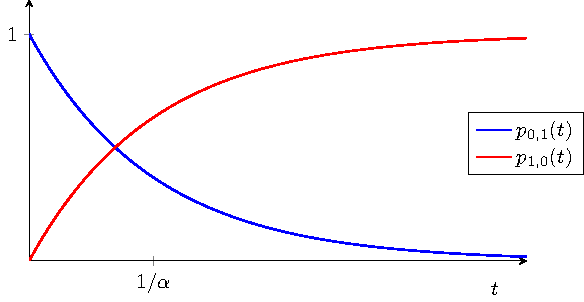
\includegraphics[width=0.62\textwidth]{figures/IMG_ch3/abs1.pdf}
\caption{State probabilities for the single-particle absorption-only model. The
particle begins outside the compartment ($p_{0,1}$, decaying exponentially at rate
$\alpha$) and ends inside it ($p_{1,0}$). There is nowhere else for it to go, so
the two curves sum to one at every time.}
\label{m:fig:abs1}
\end{figure}


\subsection{Absorption--birth--death}
\label{m:sec:absbirthdeath}

Introducing replication for particles inside the compartment, the independence
property is still present but no longer serves as a shortcut: from a single initial
particle, birth events make infinitely many states reachable, so $G_1(x,y,t)$ is an
infinite sum and there is nothing to be gained by factorising. The partial
differential equation must therefore be solved directly, and by now that can be
done.

With $X_t$ and $Y_t$ as before, birth at per-capita rate $\lambda$ is added to the
transition probabilities:
\begin{align*}
\pr{\Delta X = 1,\ \Delta Y = -1 \mid Y_t=j} &= j\alpha\,\Delta t, &&\text{(absorption)}\\
\pr{\Delta X = 1,\ \Delta Y = 0 \mid X_t=i} &= i\lambda\,\Delta t, &&\text{(birth)}\\
\pr{\Delta X = -1,\ \Delta Y = 0 \mid X_t=i} &= i\mu\,\Delta t, &&\text{(death)}\\
\pr{\Delta X = 0,\ \Delta Y = 0 \mid X_t=i,\ Y_t=j} &= 1-(j\alpha+i\mu+i\lambda)\Delta t, &&\text{(no event)}
\end{align*}
with forward Kolmogorov equation
\begin{equation}
\label{m:eq:FK3}
\ddt{p_{i,j}} = \alpha(j+1)p_{i-1,j+1} + \mu(i+1)p_{i+1,j} + \lambda(i-1)p_{i-1,j}
- (\alpha j+\mu i+\lambda i)p_{i,j} .
\end{equation}
The same reasoning as before gives the generating-function equation
\begin{equation}
\label{m:eq:PDE3}
\pddt{G} = \bigl(\mu-(\mu+\lambda)x+\lambda x^2\bigr)\pdd{G}{x} + \alpha(x-y)\pdd{G}{y},
\qquad G(x,y,0)=y^N ,
\end{equation}
whose $x$-coefficient is exactly the quadratic met in \cref{m:eq:bdpde} for the
linear birth--death process. Reparametrising $(x,y,t)\to(\sigma,\eta,\tau)$ as in
\cref{m:sec:mocabsdeath} gives the characteristic system
\begin{align}
\dda{G}{\tau} &= 0, \label{m:eq:ch21}\\
\dda{t}{\tau} &= -1, \label{m:eq:ch22}\\
\dda{x}{\tau} &= \mu-(\mu+\lambda)x+\lambda x^2, \label{m:eq:ch23}\\
\dda{y}{\tau} &= \alpha(x-y), \label{m:eq:ch24}
\end{align}
with the same initial conditions \cref{m:eq:ICpar}.

\paragraph{The equations for $G$ and $t$, \eqref{m:eq:ch21}--\eqref{m:eq:ch22}.}
As before,
\begin{equation}
\label{m:eq:GetaN2}
G(\sigma,\eta,\tau) = \eta^N,
\qquad
t = -\tau .
\end{equation}

\paragraph{The equation for $x$, \eqref{m:eq:ch23}.}
This is a Riccati equation of the same shape as the one governing the survival
probability in the continuum approximation of \ChA. Its right-hand side factorises, and the roots
are elementary rather than the surd expression that mechanical use of the quadratic
formula suggests:
\begin{equation}
\label{m:eq:xpm}
\mu-(\mu+\lambda)x+\lambda x^2 = \lambda(x-x_+)(x-x_-),
\qquad
x_+ = 1,\quad x_- = \frac{\mu}{\lambda} .
\end{equation}
The discriminant is
$\bigl(\tfrac{\mu+\lambda}{2\lambda}\bigr)^2 - \tfrac{\mu}{\lambda}
= \bigl(\tfrac{\lambda-\mu}{2\lambda}\bigr)^2$, a perfect square, so the surds
cancel. It is convenient to name the combination that appears throughout,
\begin{equation}
\label{m:eq:b1}
b_1 = \lambda(x_+-x_-) = \lambda-\mu ,
\end{equation}
the net interior growth rate. Separating variables in \cref{m:eq:ch23} and applying
\cref{m:eq:ICpar} gives the characteristic in the compact form
\begin{equation}
\label{m:eq:xratio}
\frac{x-x_+}{x-x_-} = \lrb{\frac{\sigma-x_+}{\sigma-x_-}}\ee^{b_1\tau},
\end{equation}
or, solved for $x$,
\begin{equation}
\label{m:eq:xabd}
x(\tau) = \frac{x_+(\sigma-x_-) - x_-(\sigma-x_+)\ee^{b_1\tau}}
{(\sigma-x_-) - (\sigma-x_+)\ee^{b_1\tau}} .
\end{equation}

\paragraph{The equation for $y$, \eqref{m:eq:ch24}.}
The last characteristic equation is $\dd y/\dd\tau = \alpha(x-y)$, which with an
integrating factor becomes
\begin{equation}
\label{m:eq:yint}
\dda{}{\tau}\lrb{\ee^{\alpha\tau}y} = \alpha\,\ee^{\alpha\tau}x(\tau) .
\end{equation}
The integral on the right is where the difficulty lies. Rather than substitute
\cref{m:eq:xabd} and split the resulting quotient --- which leads to two
hypergeometric integrals and a good deal of bookkeeping --- it is cleaner to expand
$x(\tau)$ first. Writing $x-x_- = (x-x_+)+(x_+-x_-)$ in \cref{m:eq:xratio} and
solving for $x$ gives
\begin{equation}
\label{m:eq:xgeom}
x(\tau) = x_+ + (x_+-x_-)\frac{\zeta(\tau)}{1-\zeta(\tau)},
\qquad
\zeta(\tau) = \lrb{\frac{\sigma-x_+}{\sigma-x_-}}\ee^{b_1\tau},
\end{equation}
so that, for $|\zeta|<1$,
\begin{equation*}
x(\tau) = x_+ + (x_+-x_-)\sum_{n=1}^{\infty}\zeta(\tau)^n .
\end{equation*}
Every term is now a pure exponential in $\tau$ and integrates immediately. Writing
$Z = (\sigma-x_+)/(\sigma-x_-)$, so that $\zeta(\tau) = Z\ee^{b_1\tau}$ and
$Z^n\ee^{nb_1\tau} = \zeta^n$,
\begin{align*}
\alpha\int\ee^{\alpha\tau}x(\tau)\,\dd\tau
&= \alpha x_+\!\int\!\ee^{\alpha\tau}\dd\tau
 + \alpha(x_+-x_-)\sum_{n=1}^{\infty}Z^n\!\int\!\ee^{(\alpha+nb_1)\tau}\dd\tau\\
&= \ee^{\alpha\tau}\lrbs{x_+ + \alpha(x_+-x_-)\sum_{n=1}^{\infty}\frac{\zeta^n}{\alpha+nb_1}}
 + \text{const} .
\end{align*}
Setting $\delta = \alpha/b_1$ and using $\alpha(x_+-x_-)/b_1 = \alpha/\lambda$ by
\cref{m:eq:b1}, this defines the function that carries the whole solution:
\begin{equation}
\label{m:eq:Psidef}
\Psi(\zeta) = x_+ + \frac{\alpha}{\lambda}\sum_{n=1}^{\infty}\frac{\zeta^{\,n}}{n+\delta},
\qquad
\delta = \frac{\alpha}{b_1} = \frac{\alpha}{\lambda-\mu} .
\end{equation}
So $\alpha\int\ee^{\alpha\tau}x(\tau)\dd\tau = \ee^{\alpha\tau}\Psi(\zeta(\tau)) + \text{const}$,
and integrating \cref{m:eq:yint} gives
$\ee^{\alpha\tau}y = \ee^{\alpha\tau}\Psi(\zeta(\tau)) + \text{const}$. The initial
condition $y(\sigma,\eta,0)=\eta$, at which $\zeta(0)=Z$, fixes the constant as
$\eta-\Psi(Z)$, so
\begin{equation}
\label{m:eq:etasolved}
\eta = \ee^{\alpha\tau}\Bigl[y-\Psi\bigl(\zeta(\tau)\bigr)\Bigr] + \Psi(Z) .
\end{equation}
Finally, put $\tau=-t$ and use \cref{m:eq:xratio}: writing
\begin{equation*}
W = \frac{x-x_+}{x-x_-}
\end{equation*}
we have $\zeta(\tau) = W$ and $Z = W\ee^{-b_1\tau} = W\ee^{b_1t}$. Substituting into
\cref{m:eq:etasolved} and applying \cref{m:eq:GetaN2} gives the solution.

\begin{proposition}[Generating function for absorption--birth--death]
\label{m:prop:Gabd}
With $x_+=1$, $x_-=\mu/\lambda$, $b_1 = \lambda-\mu$, $\delta = \alpha/b_1$,
$W = (x-x_+)/(x-x_-)$ and $\Psi$ as in \cref{m:eq:Psidef},
\begin{equation}
\label{m:eq:Gabd}
\boxed{\;
G(x,y,t) = \Bigl\{\ee^{-\alpha t}\bigl[y-\Psi(W)\bigr] + \Psi\bigl(W\ee^{b_1t}\bigr)\Bigr\}^{N}. \;}
\end{equation}
\end{proposition}

Three checks confirm the result. At $t=0$ the two $\Psi$ terms cancel and $G=y^N$,
the required initial condition. At $x=y=1$ we have $W=0$ and $\Psi(0)=x_+=1$, so
$G=1$ and probability is conserved. And setting $x=1$ alone gives
\begin{equation*}
G(1,y,t) = \bigl(\ee^{-\alpha t}y + 1-\ee^{-\alpha t}\bigr)^N,
\end{equation*}
so $Y_t\sim\text{Binomial}(N,\ee^{-\alpha t})$ --- exactly right, since the
exterior particles are absorbed independently at rate $\alpha$ and what happens
inside the compartment cannot affect them. Beyond these, \cref{m:eq:Gabd} has been
verified numerically against direct integration of the master equation
\cref{m:eq:FK3}, agreeing to around $10^{-13}$ across sub- and supercritical interior
regimes and for $N=1,2,3$.

\subsubsection*{Hypergeometric form}

The series in \cref{m:eq:Psidef} is a Gauss hypergeometric function in disguise. With
\begin{equation}
\label{m:eq:2F1def}
{}_2F_1(a,b;c;z) = \sum_{n=0}^{\infty}\frac{(a)_n(b)_n}{(c)_n}\frac{z^n}{n!},
\qquad
(q)_n = \begin{cases}1, & n=0,\\ q(q+1)\cdots(q+n-1), & n\ge1,\end{cases}
\end{equation}
where $(q)_n$ is the rising Pochhammer symbol \cite{Olver2010}, the case $a=1$,
$b=\delta$, $c=\delta+1$ collapses to a single ratio. Since $(1)_n = n!$ and
\begin{equation}
\label{m:eq:pochcancel}
\frac{(\delta)_n}{(\delta+1)_n}
= \frac{\delta(\delta+1)\cdots(\delta+n-1)}{(\delta+1)\cdots(\delta+n-1)(\delta+n)}
= \frac{\delta}{\delta+n},
\end{equation}
we have
\begin{equation}
\label{m:eq:2F1simple}
{}_2F_1(1,\delta;\delta+1;z) = \sum_{n=0}^{\infty}\frac{\delta}{\delta+n}z^n .
\end{equation}
Comparing with \cref{m:eq:Psidef} and using
$\alpha/(\lambda\delta) = b_1/\lambda = x_+-x_-$,
\begin{equation}
\label{m:eq:Psihyp}
\Psi(\zeta) = x_+ + (x_+-x_-)\Bigl[{}_2F_1(1,\delta;\delta+1;\zeta)-1\Bigr] .
\end{equation}
\Cref{m:eq:Gabd} together with \cref{m:eq:Psihyp} is the closed form. It is not pretty,
but it is a genuine closed form in terms of a standard special function, and the
elementary series \cref{m:eq:Psidef} is what one would actually evaluate. An
alternative derivation of the same object, by way of the integral
$\int\ee^{h\tau}/(P+Q\ee^{k\tau})\,\dd\tau$, is given in \cref{m:app:hyp}; that route
is longer, but it produces a general identity of independent use.

\begin{remark}[Domain of validity]
\label{m:rem:domain}
The series \cref{m:eq:Psidef} converges for $|\zeta|<1$, and the arguments appearing
in \cref{m:eq:Gabd} are $W$ and $W\ee^{b_1t}$. In the subcritical interior regime
$\mu>\lambda$ we have $b_1<0$ and $x_- = \mu/\lambda>1$, so for $x\in[0,1]$ the
argument $W$ lies in $[0,\lambda/\mu]\subset[0,1)$ and $W\ee^{b_1t}$ is smaller
still: the series representation is valid on the whole of the unit square, which is
the case of most interest here. When $\lambda>\mu$ the series converges only for
$x$ above the smaller fixed point $\mu/\lambda$, and elsewhere one must use the
analytic continuation of ${}_2F_1$ --- conveniently, the Euler integral
\begin{equation*}
{}_2F_1(1,\delta;\delta+1;\zeta) = \delta\int_0^1\frac{u^{\delta-1}}{1-\zeta u}\,\dd u
\qquad(\delta>0,\ \zeta\notin[1,\infty)),
\end{equation*}
which was used for the numerical verification quoted above.
\end{remark}

\begin{remark}[Resonance]
\label{m:rem:resonance}
The denominators in \cref{m:eq:Psidef} vanish when $n+\delta=0$ for some integer
$n\ge1$, that is when
\begin{equation*}
\alpha = n(\mu-\lambda),\qquad n=1,2,\dots
\end{equation*}
This is the classical resonance condition for linearising the $y$-equation: the
decay rate $\alpha$ of the absorption channel coincides with a harmonic of the
interior relaxation rate $\mu-\lambda$. The generating function itself is perfectly
regular there, being analytic in all parameters, so the singularity is removable,
and at resonance the corresponding term acquires a factor $\tau$ --- a secular term
--- in place of the simple exponential. The resonant parameter values form a set of
measure zero and the limit may be taken numerically, but the degeneracy should be
kept in mind when $\alpha$ happens to sit near an integer multiple of $\mu-\lambda$.
\end{remark}


\subsubsection*{Parameter-regular form and resonance}
\label{m:sec:moc-resonance}

The closed form \cref{m:eq:Gabd} can be rewritten so that the apparent singularity
at resonant parameter values is removable. When the hypergeometric parameters meet
a non-positive integer resonance, the series representation degenerates and the
correct finite limit must be taken separately; the underlying characteristic
solution remains regular. In practice one evaluates the parameter-regular
expression (or takes the resonant limit of the hypergeometric form) rather than
trusting a na\"ive specialisation of intermediate formulae. Domains of the
hypergeometric representation and the resonant cases are recorded in the source
derivations; the identities of \cref{m:app:hyp} cover the integral manipulations
used above.



\section{An integral identity for the hypergeometric function}
\label{m:app:hyp}

The route to \cref{m:eq:Psidef} taken in \cref{m:sec:absbirthdeath} expands the
characteristic $x(\tau)$ in a geometric series and integrates term by term. An
alternative is to integrate the quotient \cref{m:eq:xabd} directly, splitting the
numerator into two pieces, each of the form
\begin{equation}
\label{m:eq:Iform}
I(\tau) = \int\frac{\ee^{h\tau}}{P+Q\,\ee^{k\tau}}\,\dd\tau
\end{equation}
with $h,k,P,Q$ constant. That route is longer and easier to get wrong --- the two
pieces carry different prefactors, and dropping one produces a formula that still
satisfies the initial condition while violating $G(1,1,t)=1$ --- but the identity it
rests on is useful in its own right, so it is recorded and proved here.

\begin{proposition}
\label{m:prop:hypIden}
For $h/k>0$ and $-\tfrac{Q}{P}\ee^{k\tau}\notin[1,\infty)$,
\begin{equation}
\label{m:eq:hypIden}
\int\frac{\ee^{h\tau}}{P+Q\ee^{k\tau}}\,\dd\tau
= \frac{\ee^{h\tau}}{Ph}\,{}_2F_1\lrb{1,\frac{h}{k};\frac{h}{k}+1;\,-\frac{Q}{P}\ee^{k\tau}}
+ \text{const} .
\end{equation}
\end{proposition}

\begin{proof}
We use the Euler integral representation of the hypergeometric function
\cite{Olver2010},
\begin{equation}
\label{m:eq:idenHyp}
{}_2F_1(a,b;c;z)
= \frac{\Gamma(c)}{\Gamma(b)\Gamma(c-b)}\int_0^1 u^{b-1}(1-u)^{c-b-1}(1-zu)^{-a}\,\dd u ,
\end{equation}
$\Gamma$ being the gamma function.

Start from \cref{m:eq:Iform} and substitute $v = \ee^{k\tau}$, so that
$\dd\tau = k^{-1}v^{-1}\dd v$:
\begin{equation*}
I = \frac1k\int\frac{v^{h/k}}{P+Qv}\,v^{-1}\dd v
= \frac{1}{Pk}\int\frac{v^{h/k-1}}{1+\frac{Q}{P}v}\,\dd v .
\end{equation*}
Fix the antiderivative by writing this as a definite integral from $0$ to $v$ in a
dummy variable $w$; the integral converges at the lower limit precisely because
$h/k>0$:
\begin{equation*}
I = \frac{1}{Pk}\int_0^v\frac{w^{h/k-1}}{1+\frac{Q}{P}w}\,\dd w .
\end{equation*}
Now rescale, $w = vu$, so that $\dd w = v\,\dd u$ with $v$ held fixed:
\begin{equation}
\label{m:eq:backat}
I = \frac{1}{Pk}\int_0^1\frac{(vu)^{h/k-1}}{1+\frac{Q}{P}vu}\,v\,\dd u
= \frac{v^{h/k}}{Pk}\int_0^1\frac{u^{h/k-1}}{1+\frac{Q}{P}vu}\,\dd u .
\end{equation}
The remaining integrand matches that of \cref{m:eq:idenHyp} with $b = h/k$,
$c = h/k+1$, $a=1$ and $z = -\tfrac{Q}{P}v$, since then $(1-u)^{c-b-1} = 1$ and
$(1-zu)^{-a} = \bigl(1+\tfrac{Q}{P}vu\bigr)^{-1}$. Hence, using
$\Gamma(z+1) = z\Gamma(z)$,
\begin{equation*}
\int_0^1\frac{u^{h/k-1}}{1+\frac{Q}{P}vu}\,\dd u
= \frac{\Gamma\!\lrb{\frac hk}\Gamma(1)}{\Gamma\!\lrb{\frac hk+1}}\,
{}_2F_1\lrb{1,\frac hk;\frac hk+1;-\frac QP v}
= \frac kh\,{}_2F_1\lrb{1,\frac hk;\frac hk+1;-\frac QP v}.
\end{equation*}
Substituting into \cref{m:eq:backat} gives
\begin{equation*}
I = \frac{v^{h/k}}{Ph}\,{}_2F_1\lrb{1,\frac hk;\frac hk+1;-\frac QP v},
\end{equation*}
and restoring $v = \ee^{k\tau}$ gives \cref{m:eq:hypIden}.
\end{proof}

\begin{remark}
Applied to the two pieces of \cref{m:eq:xabd} --- the first with $h=\alpha$, the
second with $h = \alpha+b_1$, and both with $k=b_1$, $P = \sigma-x_-$ and
$Q = -(\sigma-x_+)$ --- \cref{m:prop:hypIden} reproduces \cref{m:eq:Psihyp} once the
prefactors $\alpha x_+(\sigma-x_-)$ and $-\alpha x_-(\sigma-x_+)$ are carried
through correctly. The factor $(\sigma-x_+)/(\sigma-x_-)$ attached to the second
piece is easily lost, and its loss is invisible at $t=0$; checking $G(1,1,t)=1$
catches it immediately.
\end{remark}

\section{Extracting state probabilities from a generating function}
\label{m:app:extract}

A generating function defined by a formula rather than as an explicit series --- for
example
\begin{equation}
\label{m:eq:examplePgf}
G(x,y,t) = \Bigl(\bigl(1-\ee^{-\alpha t}\bigr)x + \ee^{-\alpha t}y\Bigr)^n
\end{equation}
--- can always be converted back to the form
\begin{equation}
\label{m:eq:series1}
G(x,y,t) = \sum_{i=0}^{\infty}\sum_{j=0}^{\infty}p_{i,j}(t)\,x^iy^j ,
\end{equation}
recovering the time-dependent state probabilities. All that is required is that $G$
be repeatedly partially differentiable in $x$ and $y$.

The reason is the bivariate Maclaurin expansion,
\begin{equation*}
f(x,y) = \sum_{k=0}^{\infty}\frac{1}{k!}\sum_{\varrho=0}^{k}\binom{k}{\varrho}
\partial_x^{\varrho}\partial_y^{\,k-\varrho}f\Big|_{(0,0)}\;x^{\varrho}y^{k-\varrho},
\end{equation*}
whose coefficient of $x^iy^j$, taking $k=i+j$ and $\varrho=i$, is
$\frac{1}{(i+j)!}\binom{i+j}{i}\partial_x^i\partial_y^{\,j}f\big|_{(0,0)}$. Hence
\begin{equation}
\label{m:eq:stateProb}
p_{i,j}(t) = \frac{1}{i!\,j!}\,\partial_x^i\partial_y^{\,j}G\Big|_{(0,0)} .
\end{equation}

\subsection*{The multilinear case}

Both \cref{m:eq:Gabsonly} and \cref{m:eq:Gabsdeath} have the form
\begin{equation}
\label{m:eq:multilinear}
G(x,y,t) = \bigl(c(t) + f(t)\,x + g(t)\,y\bigr)^n ,
\end{equation}
for which the derivatives are immediate. Each differentiation lowers the power by
one and brings down a factor, so
\begin{equation}
\label{m:eq:derivs}
\partial_x^{a}\partial_y^{\,b}G
= \frac{n!}{(n-a-b)!}\,f^{a}g^{b}\bigl(c+fx+gy\bigr)^{n-a-b}
\qquad(a+b\le n),
\end{equation}
and zero for $a+b>n$. Evaluating at the origin and applying \cref{m:eq:stateProb},
\begin{equation}
\label{m:eq:stateProbSpec}
p_{i,j}(t) = \frac{n!}{i!\,j!\,(n-i-j)!}\;f(t)^{i}g(t)^{j}c(t)^{\,n-i-j},
\qquad i+j\le n,
\end{equation}
and $p_{i,j}=0$ otherwise. This is the trinomial distribution, which is exactly
what it should be: the $n$ particles are independent, and at time $t$ each is in
one of three states, with probabilities $c$ (neither inside nor outside --- that
is, dead), $f$ (inside) and $g$ (outside). Note in particular that the falling
factorial $n!/(n-i-j)!$ in \cref{m:eq:derivs} is \emph{not} $n^{i+j}$; the two agree
only to leading order in $n$, and using the latter breaks normalisation.

\subsection*{Applied to the absorption models}

For absorption only, \cref{m:eq:examplePgf}, we have $c=0$, $f = 1-\ee^{-\alpha t}$
and $g = \ee^{-\alpha t}$. The factor $c^{\,n-i-j}$ then vanishes unless $i+j=n$,
and \cref{m:eq:stateProbSpec} gives
\begin{equation*}
p_{i,j}(t) = \binom{n}{i}\bigl(1-\ee^{-\alpha t}\bigr)^{i}\bigl(\ee^{-\alpha t}\bigr)^{j},
\qquad i+j=n,
\end{equation*}
so $X_t\sim\text{Binomial}\bigl(n,1-\ee^{-\alpha t}\bigr)$ and $Y_t = n-X_t$, as
anticipated in \cref{m:sec:absonly}.

For absorption--death, \cref{m:eq:Gabsdeath}, the three functions are
\begin{equation*}
c(t) = 1-\frac{\mu}{\mu-\alpha}\ee^{-\alpha t} + \frac{\alpha}{\mu-\alpha}\ee^{-\mu t},
\qquad
f(t) = \frac{\alpha}{\mu-\alpha}\bigl(\ee^{-\alpha t}-\ee^{-\mu t}\bigr),
\qquad
g(t) = \ee^{-\alpha t},
\end{equation*}
which are precisely $p_{0,0}$, $p_{1,0}$ and $p_{0,1}$ of
\cref{m:eq:absdeathstates}, so that
\begin{equation*}
p_{i,j}(t) = \frac{n!}{i!\,j!\,(n-i-j)!}\;f(t)^{i}g(t)^{j}c(t)^{\,n-i-j} .
\end{equation*}
Each particle independently ends up dead, absorbed, or still outside, with those
three probabilities, and the joint law is trinomial. That the generating function
factorises in this way is \cref{m:eq:indRelPGF} read backwards.

The absorption--birth--death generating function of \cref{m:prop:Gabd} is not of the
form \cref{m:eq:multilinear}, and there \cref{m:eq:stateProb} must be applied to
\cref{m:eq:Gabd} directly, or the coefficients extracted numerically by Cauchy
integrals on circles $|x|=|y|=\varrho<1$.

% --- restore default section numbering for subsequent chapters --------------
\renewcommand{\thesection}{\thechapter.\arabic{section}}
